In order to discern between reliable and unreliable messages, we have considered
a bar chart of frequency of users that tweeted the most with a hover tool to
show the most frequent words spoken by each user.
Figure~\ref{fig:most_freq_users} shows the unfiltered distribution, in which the
red bars represent users that are probably sellers since their messages include
too many words like ``\emph{deal}'', ``\emph{offer}'', ``\emph{opportunity}'',
``\emph{chances}'', etc. All tweets from those users have therefore been
discarded.

\begin{figure}[!h]
    \centering
    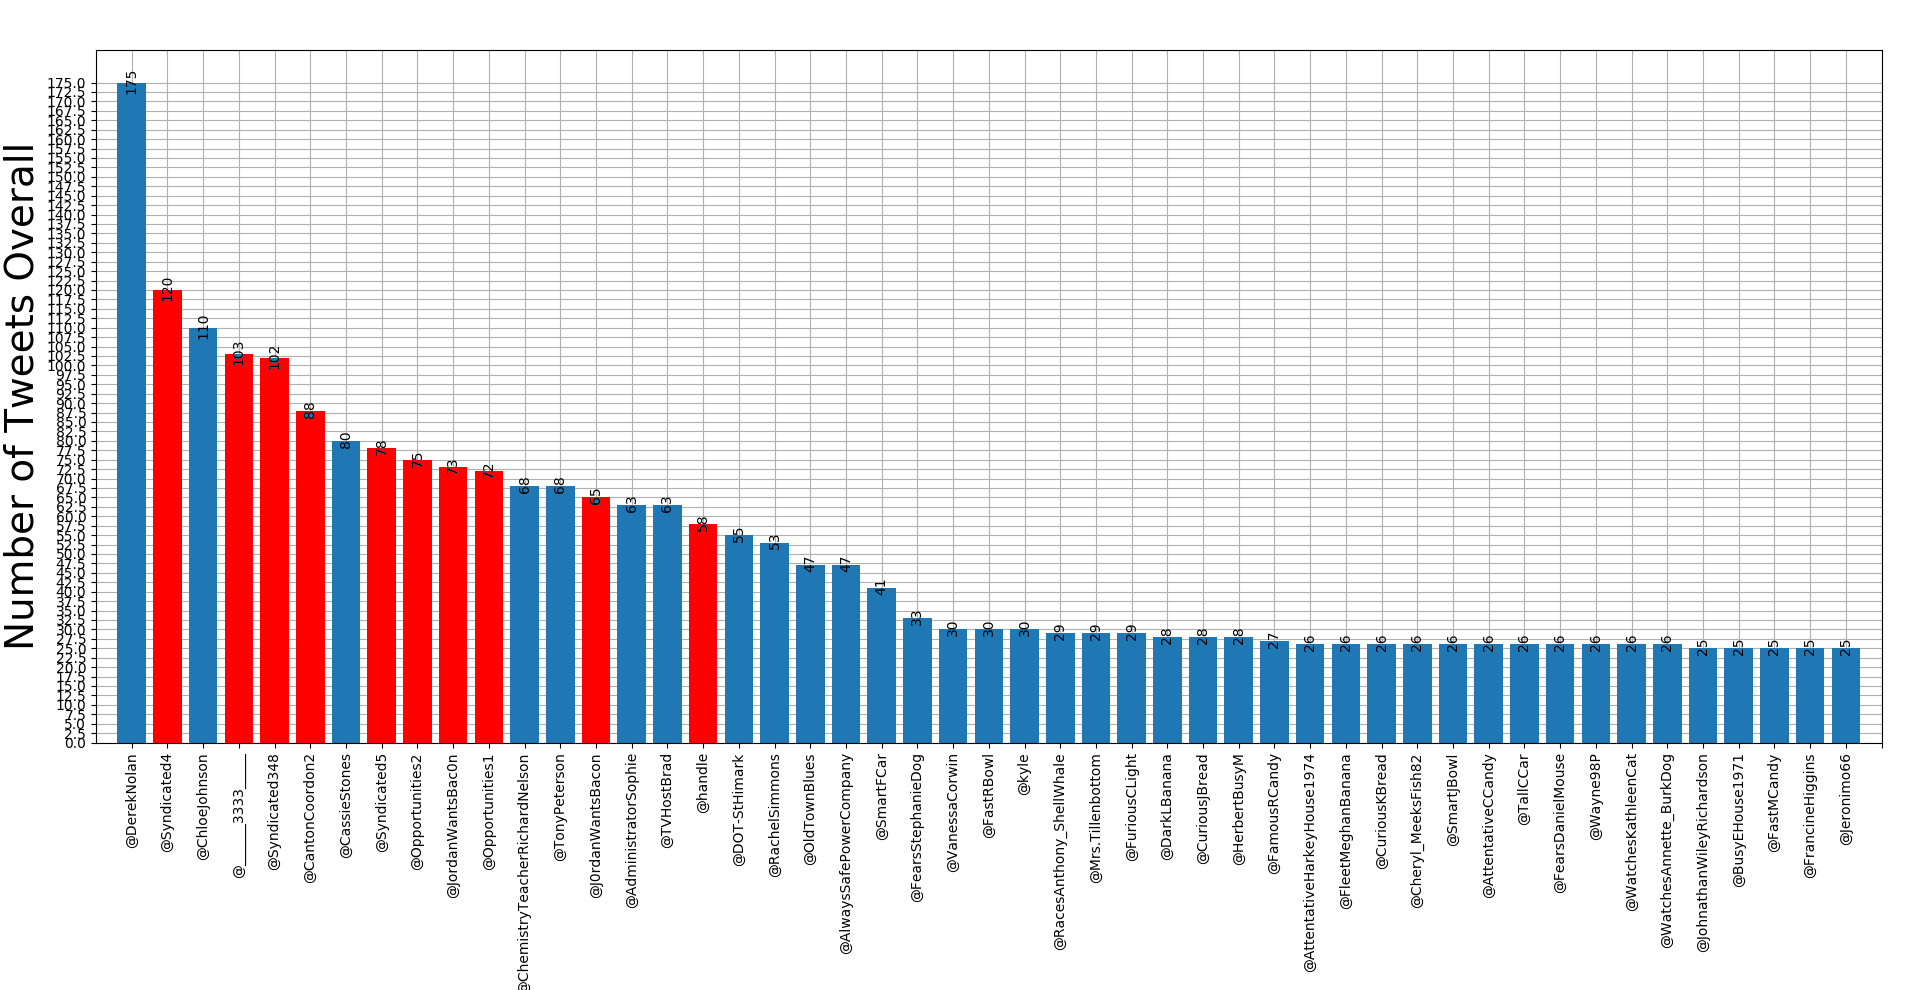
\includegraphics[width=0.95\textwidth]{figs/q1/most_freq_users.png}
    \caption{Most frequent tweeters (usernames). Red bars represent sellers.}
    \label{fig:most_freq_users}
\end{figure}

We have then counted the number of tweets per a small time interval and
presented in a histogram-like plot of Figure~\ref{fig:freq_tweet_overall} that 
shows four peaks, where things possibly might have changed across the city.

\begin{figure}[!h]
    \centering
    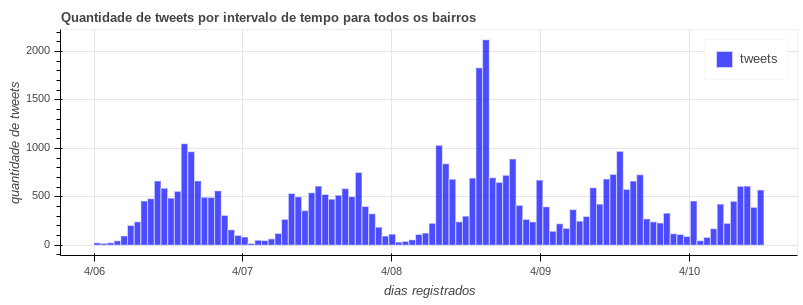
\includegraphics[width=0.95\textwidth]{figs/q1/freq_tweet_overall.png}
    \caption{Overall frequency of tweets over time considering all locations.}
    \label{fig:freq_tweet_overall}
\end{figure}

By analysing the heatmap in Figure~\ref{fig:eq_start_heat}, there appears to
have occurred three earthquakes, but the first one seems to have started at 2~PM
of the first day (April 6th). The heatmap is divided by a time interval of one
hour and by neighbourhood location. It was generated by considering a list of
keywords that were tweeted and are similar in meaning (synonyms) and are
directly related to the word ``earthquake''. The list is: 
``\emph{shake}'', ``\emph{shudder}'', ``\emph{vibrate}'', ``\emph{wobble}'',
``\emph{tremor}'', ``\emph{tremble}'', ``\emph{quaver}'', ``\emph{quiver}'',
``\emph{hazard}'', ``\emph{disaster}'', ``\emph{destruction}'', and
``\emph{rubble}''.

\begin{figure}[!h]
    \centering
    \begin{subfigure}[!h]{0.95\textwidth}
        \centering
        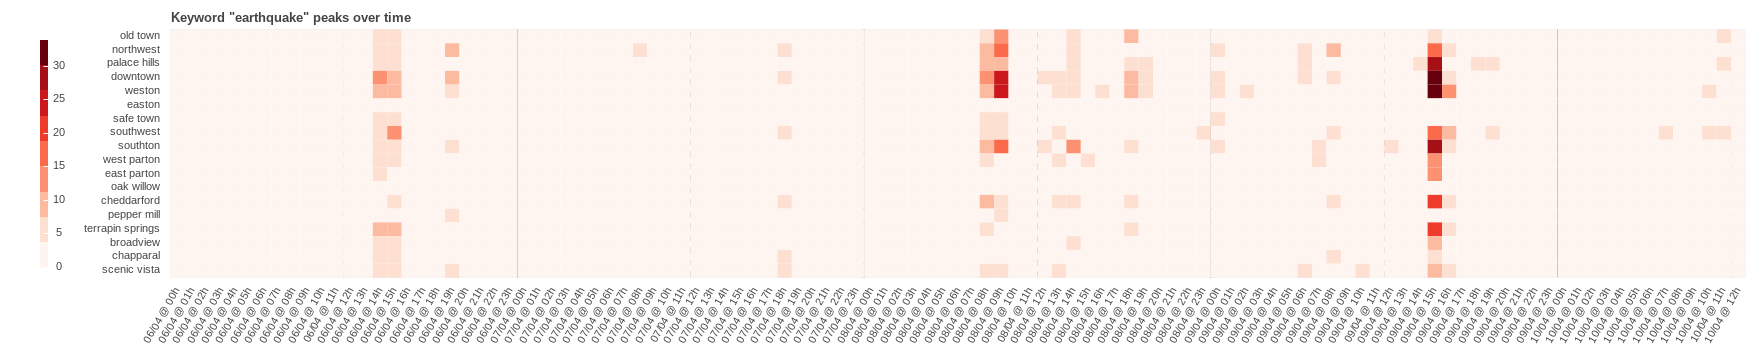
\includegraphics[width=1.00\textwidth]{figs/q1/eq_start_heat.png}
        \caption{Heatmap considering cluster of similar keywords (synonyms) for
        the word ``earthquake''.}
        \label{fig:eq_start_heat}
    \vspace{12pt}
    \end{subfigure}
    \begin{subfigure}[!h]{0.95\textwidth}
        \centering
        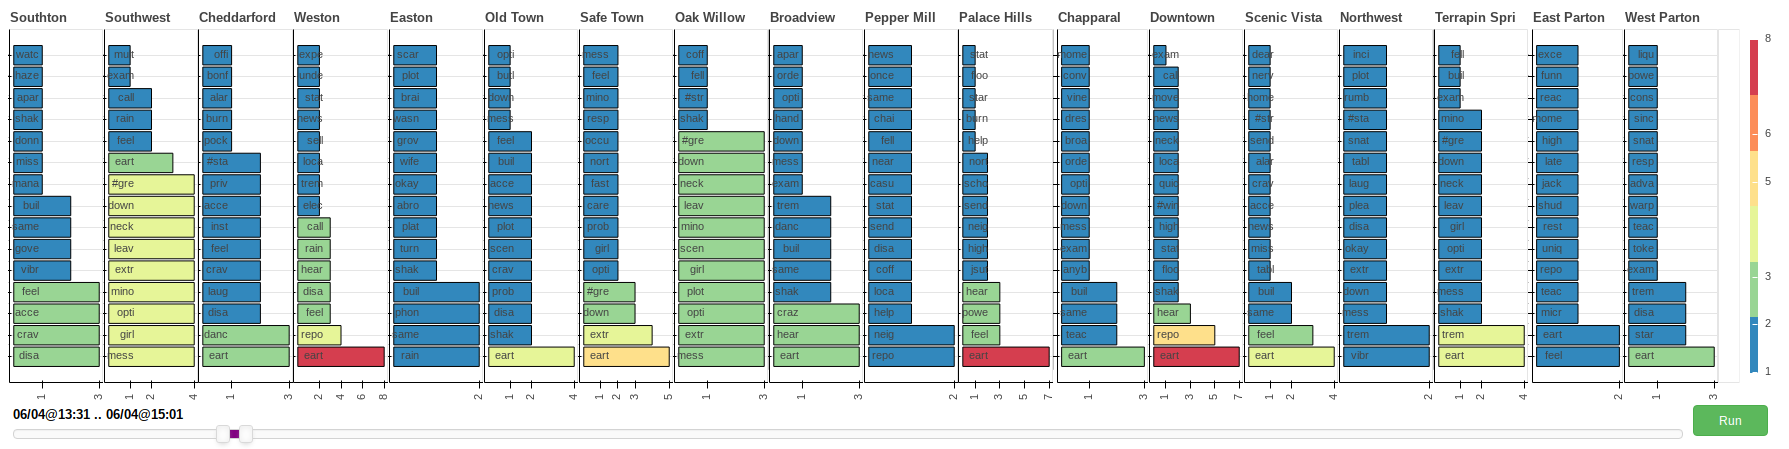
\includegraphics[width=1.00\textwidth]{figs/q1/eq_start_hbar.png}
        \caption{Bar chart with blue-to-red colormap considering frequency of
        words from 1:00~PM to 3:00~PM of April 6th.}
        \label{fig:eq_start_hbar}
    \end{subfigure}
    \caption{Conditions at the start of the earthquake.}
    \label{fig:eq_start}
\end{figure}

To ensure the heatmap is providing a reliable information, a horizontal bar
chart, shown in Figure~\ref{fig:eq_start_hbar}, was used from 1:30~PM to 
3:00~PM. It counts isolated words and discards words such as adverbs, pronouns,
adjectives, articles and some nouns and verbs that were considered to be useless
such as ``anyone'', ``make'', ``know'', ``food'', ``hate'', etc. Then the Porter
Stemmer from the \texttt{nltk} package was used to clip the words by its
invariant parts (word root), and that root was further reduced to 4-chars only.
A heat-like colormap from blue to red was also included to enhance frequency
distinction. 

The bar chart shows some interesting other words such as ``\emph{feel}'',
``\emph{hear}'', ``\emph{report}'' apart from the keywords aforementioned, in
which ``\emph{earthquake}'' is the most frequent one in accordance with the red
color.

Figure~\ref{fig:map_5h} shows a dynamically-colored SVG map of the city, where
the neighbourhood inner colors range from blue to red in a heatmap fashion
according to the average mean of the colors of the five bigger bars of the
horizontal bar chart of Figure~\ref{fig:eq_start_hbar} for each location. It
appears most reports come from the northwest and southeast of the city.

\begin{figure}[!h]
    \centering
    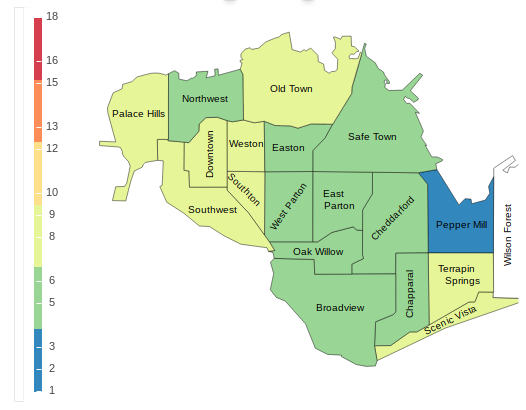
\includegraphics[width=0.50\textwidth]{figs/q1/cond_5h/cond_5h_svg.png}
    \caption{St. Himark's map 5h after the first earthquake. Lighter shades of
    green represent a higher frequency of messages.}
    \label{fig:map_5h}
\end{figure}

Figure~\ref{fig:eq_cond_5h} shows multiple heatmaps, one per keyword, in a
five-hour time interval from 2:00~PM to 6:59~PM. The charts at the top show
three blank graphs for the keywords ``building'' (Figure~\ref{fig:build_5h}),
``medical'' (Figure~\ref{fig:medical_5h}), and ``road''
(Figure~\ref{fig:road_5h}), which means these resources do not appear to be
requested by any neighbourhood. On the other hand, the 3 graphs at the bottom
show the number of mentions for keywords related to ``sewer and water''
(Figure~\ref{fig:sewer_5h}), ``power'' (Figure~\ref{fig:power_5h}), and ``rain''
(Figure~\ref{fig:rain_5h}).

\begin{figure}[!h]
    \centering
    \begin{subfigure}[!h]{0.32\textwidth}
        \centering
        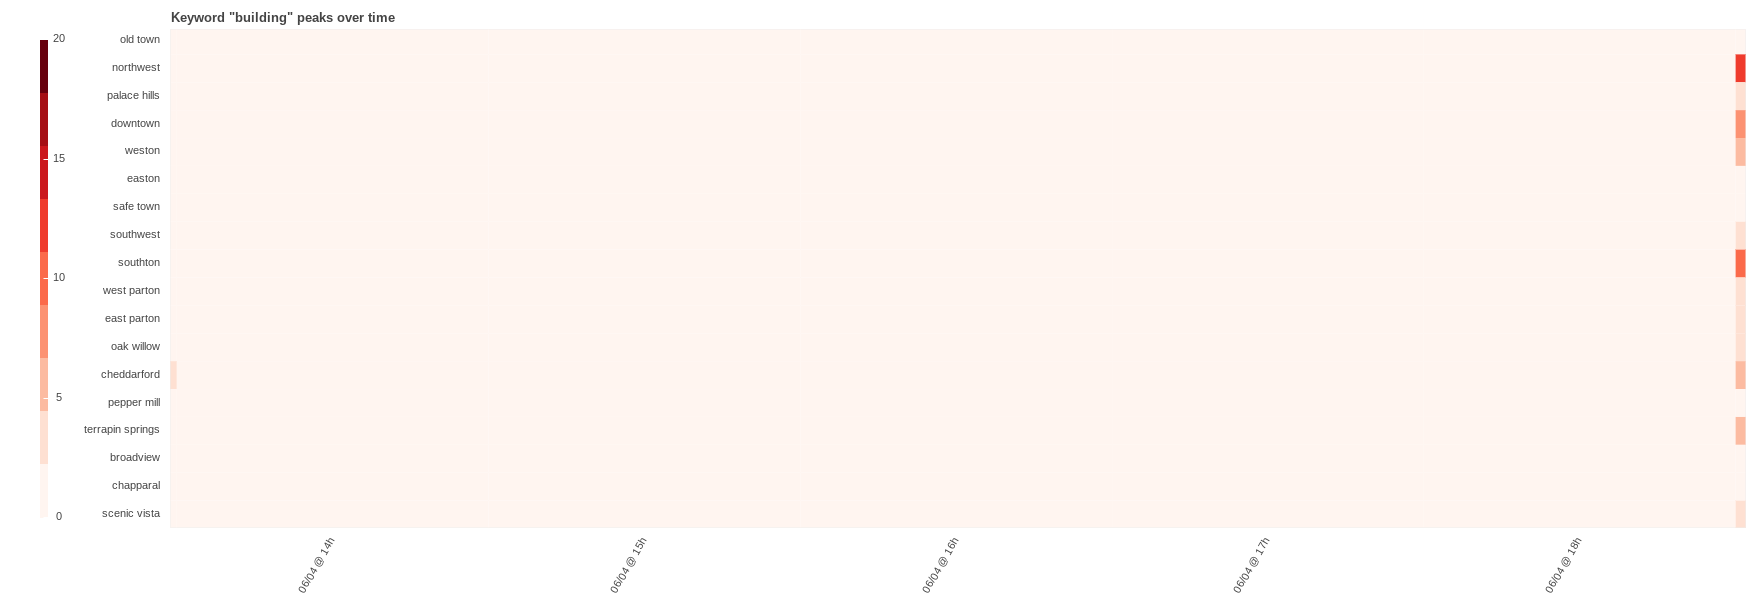
\includegraphics[width=1.00\textwidth]{figs/q1/cond_5h/cond_5h_build.png}
        \caption{Building}
        \label{fig:build_5h}
    \end{subfigure}
    \begin{subfigure}[!h]{0.32\textwidth}
        \centering
        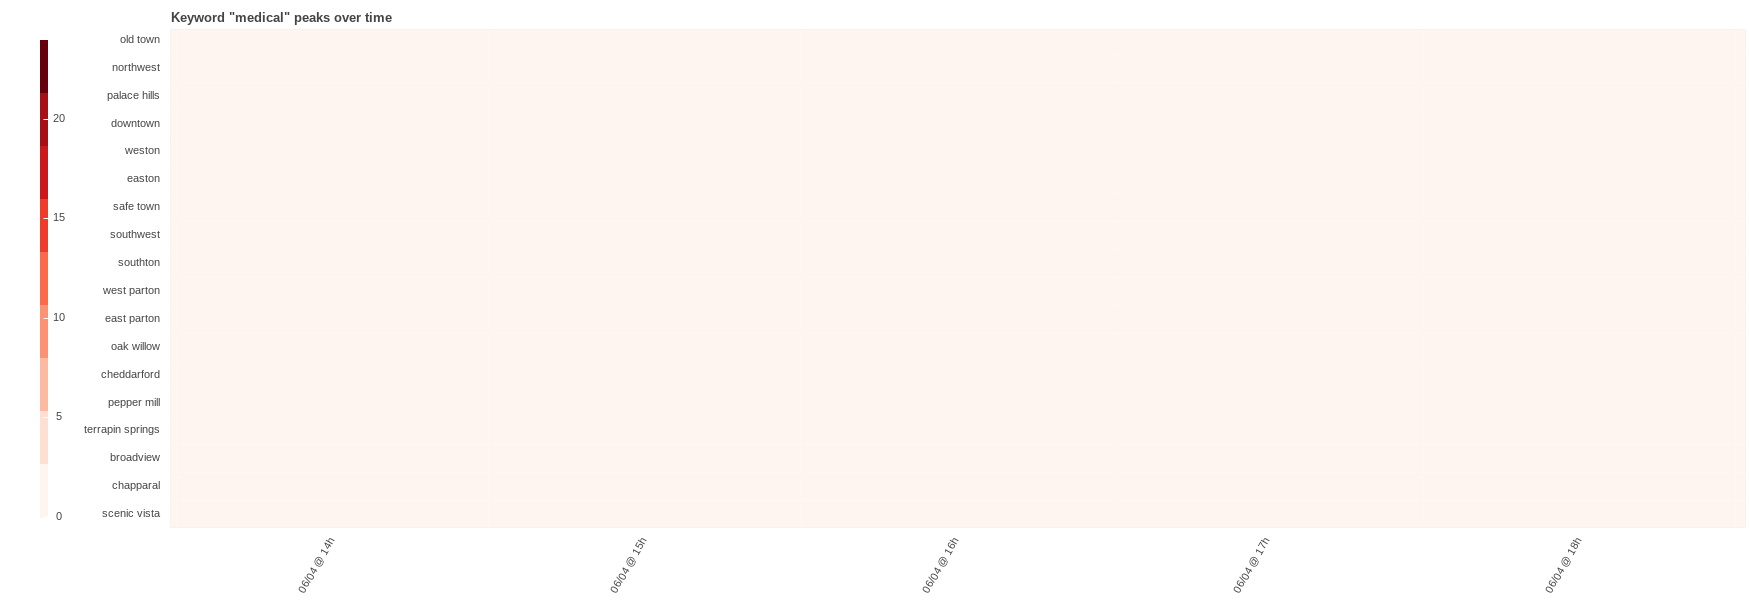
\includegraphics[width=1.00\textwidth]{figs/q1/cond_5h/cond_5h_medical.png}
        \caption{Medical}
        \label{fig:medical_5h}
    \end{subfigure}
    \begin{subfigure}[!h]{0.32\textwidth}
        \centering
        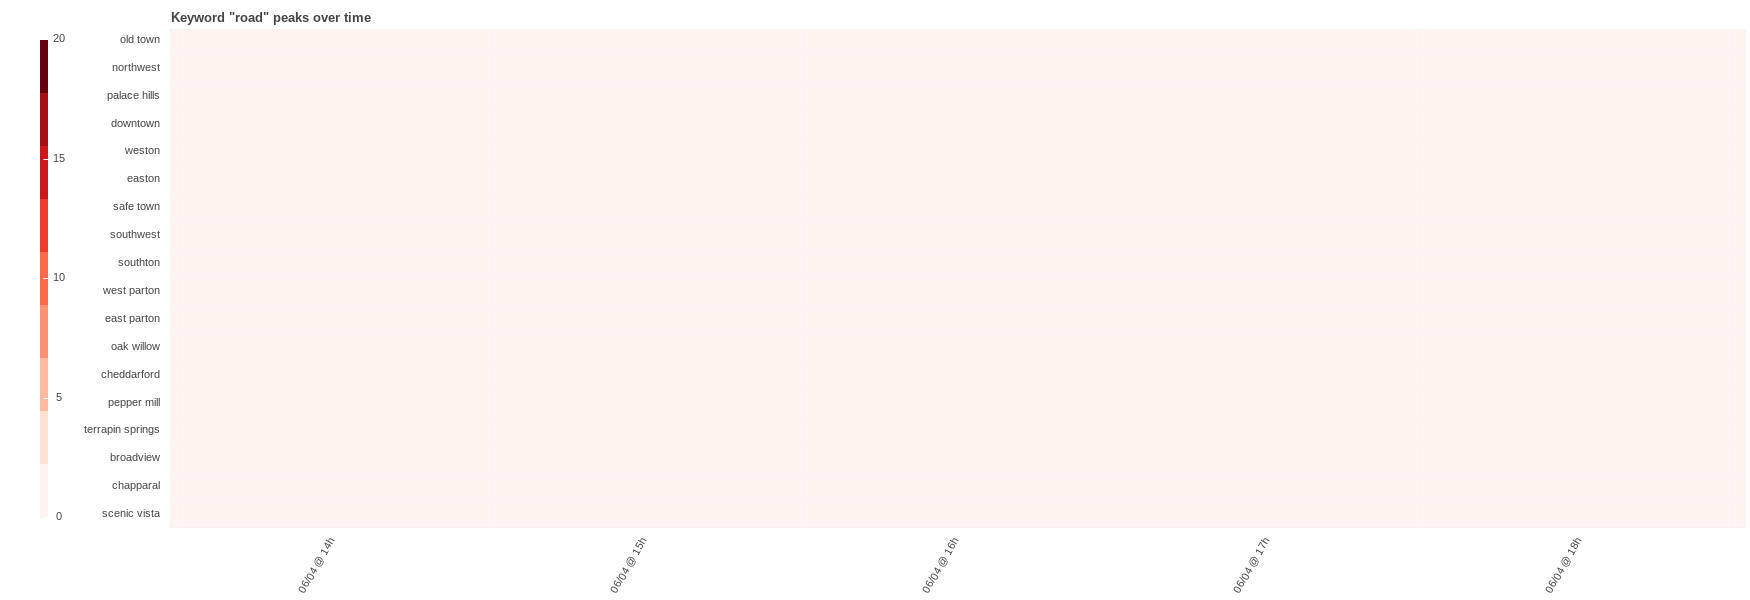
\includegraphics[width=1.00\textwidth]{figs/q1/cond_5h/cond_5h_road.png}
        \caption{Roads and Bridges}
        \label{fig:road_5h}
    \end{subfigure}
    \begin{subfigure}[!h]{0.32\textwidth}
        \centering
        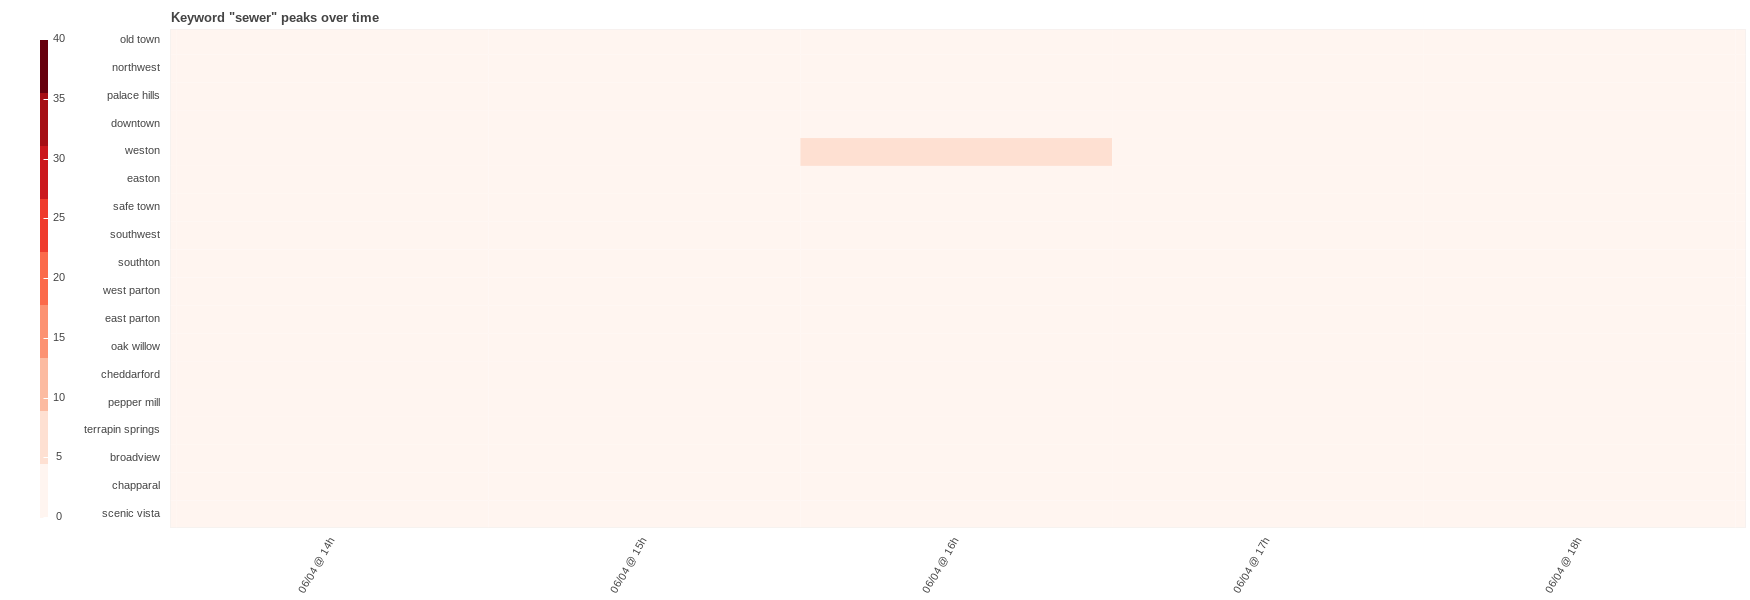
\includegraphics[width=1.00\textwidth]{figs/q1/cond_5h/cond_5h_sewer.png}
        \caption{Sewer and water}
        \label{fig:sewer_5h}
    \end{subfigure}
    \begin{subfigure}[!h]{0.32\textwidth}
        \centering
        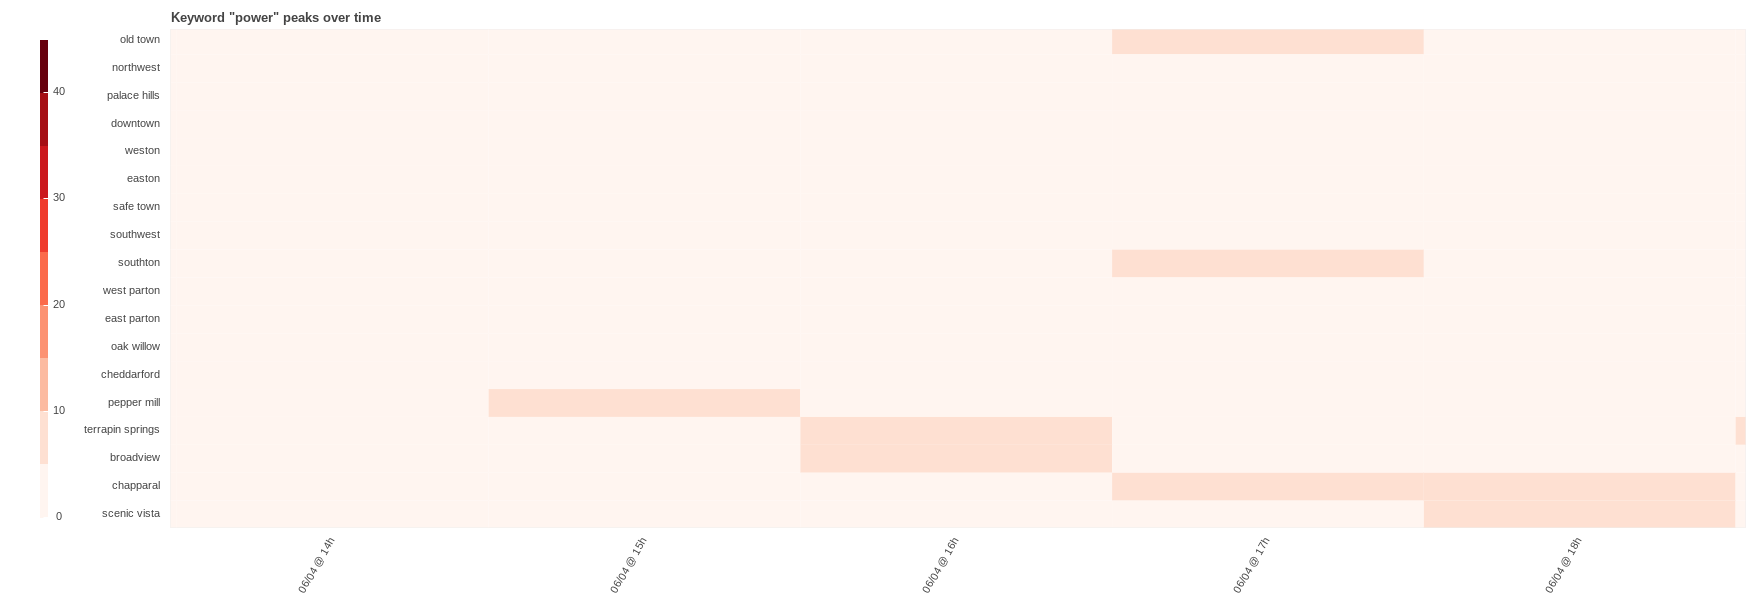
\includegraphics[width=1.00\textwidth]{figs/q1/cond_5h/cond_5h_power.png}
        \caption{Power}
        \label{fig:power_5h}
    \end{subfigure}
    \begin{subfigure}[!h]{0.32\textwidth}
        \centering
        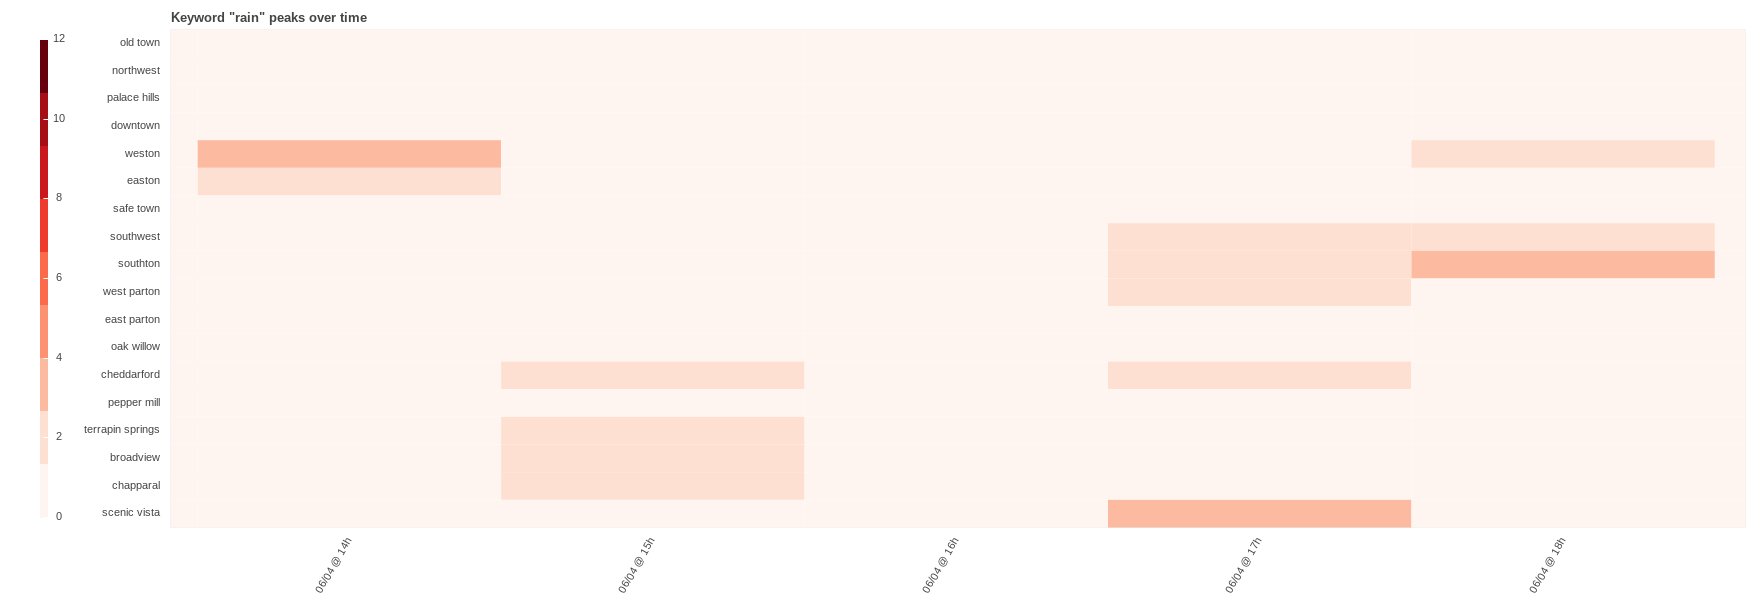
\includegraphics[width=1.00\textwidth]{figs/q1/cond_5h/cond_5h_rain.png}
        \caption{Rain}
        \label{fig:rain_5h}
    \end{subfigure}
    \caption{Conditions after 5h of the first earthquake}
    \label{fig:eq_cond_5h}
\end{figure}

Suggestions for crew allocation is detailed as follows: 

\begin{itemize}
    \item \emph{Sewer and water:} A crew must be sent only to Weston between 
    4:00~PM and 4:59~PM.
    \smallskip 
    \item \emph{Power}: Issues have occurred in Pepper Mill, \textbf{Terrapin
    Springs}, \textbf{Broadview}, Chapparal, \textbf{Southton}, \textbf{Old 
    Town} and Scenic Vista, but we'll consider only the locations 
    highlighted in bold because they have hospitals.
    \begin{itemize}
        \item A crew must be sent to Terrapin Springs between 3:00~PM and
        3:59~PM. Broadview also has a power demand at this time interval but the
        tweet frequency is much lower considering the five-hour period.
        \item Two crews must be sent to Old Town and Southton between 4:00~PM 
        and 4:59~PM.
        \item Lastly, the crew from Terrapin Springs can be reallocated to
        Chapparal between 5:00~PM and 5:59~PM. Although Chapparal does not have
        hospitals, it has been nearly two hours with electrical issues.
    \end{itemize}
    \item \emph{Rescue, sewer and water}: A crew must be sent to Southton only
    because there have been small issues in Weston, Southton and Downtown, and
    therefore Southton is geographically in the middle of such neighbourhoods.
\end{itemize}

Looking at the useful-words colormap over the SVG map of St. Hirmak, shown in
Figure~\ref{fig:map_30h}, it can be
inferred right at the outset that the neighbourhoods that are in most need are
Downtown, Southton, Old Town and Weston.

\begin{figure}[!h]
    \centering
    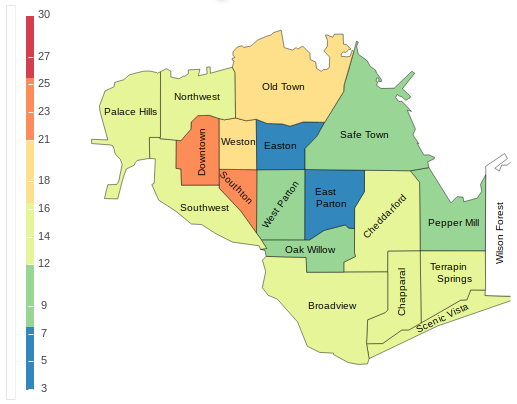
\includegraphics[width=0.50\textwidth]{figs/q1/cond_30h/cond_30h_svg.png}
    \caption{St. Himark's map 30h after the first earthquake. Yellow and orange 
    shades represent a higher frequency of messages.}
    \label{fig:map_30h}
\end{figure}

\begin{figure}[!h]
    \centering
    \begin{subfigure}[!h]{0.24\textwidth}
        \centering
        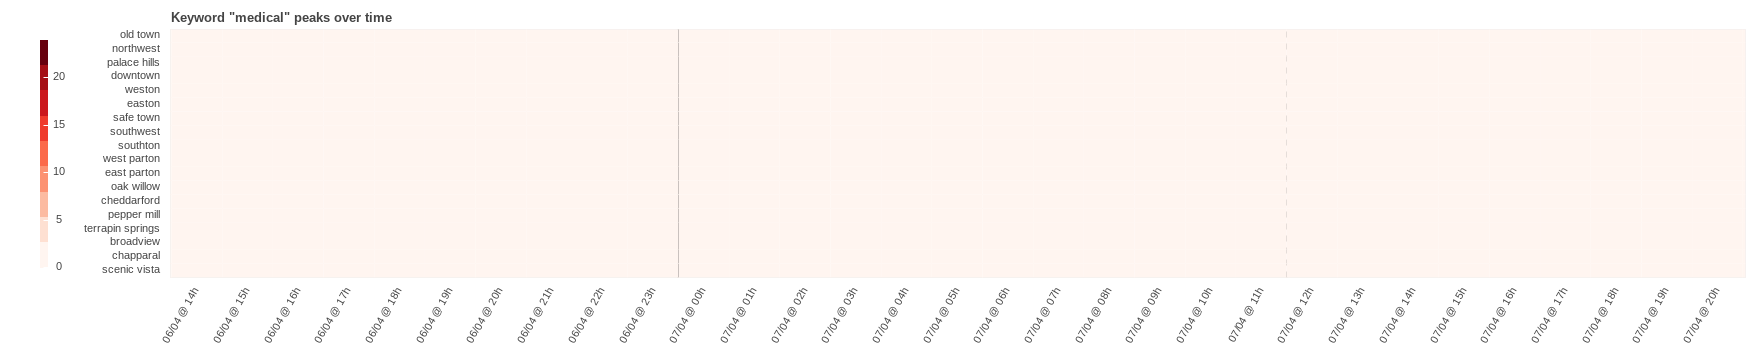
\includegraphics[width=1.00\textwidth]{figs/q1/cond_30h/cond_30h_medical.png}
        \caption{Medical}
        \label{fig:medical_30h}
    \end{subfigure}
    \begin{subfigure}[!h]{0.24\textwidth}
        \centering
        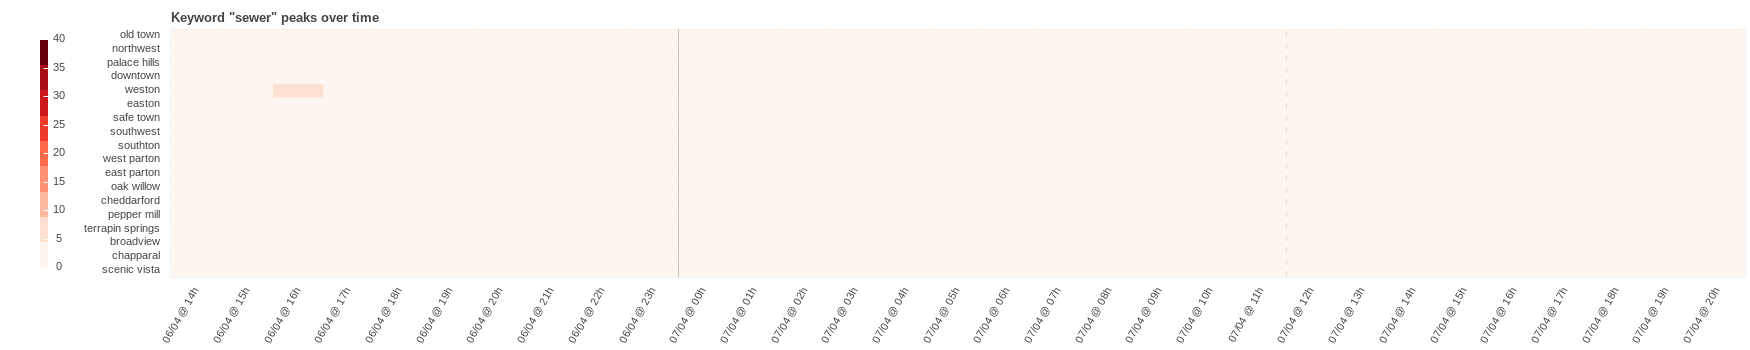
\includegraphics[width=1.00\textwidth]{figs/q1/cond_30h/cond_30h_sewer.png}
        \caption{Sewer and water}
        \label{fig:sewer_30h}
    \end{subfigure}
    \begin{subfigure}[!h]{0.24\textwidth}
        \centering
        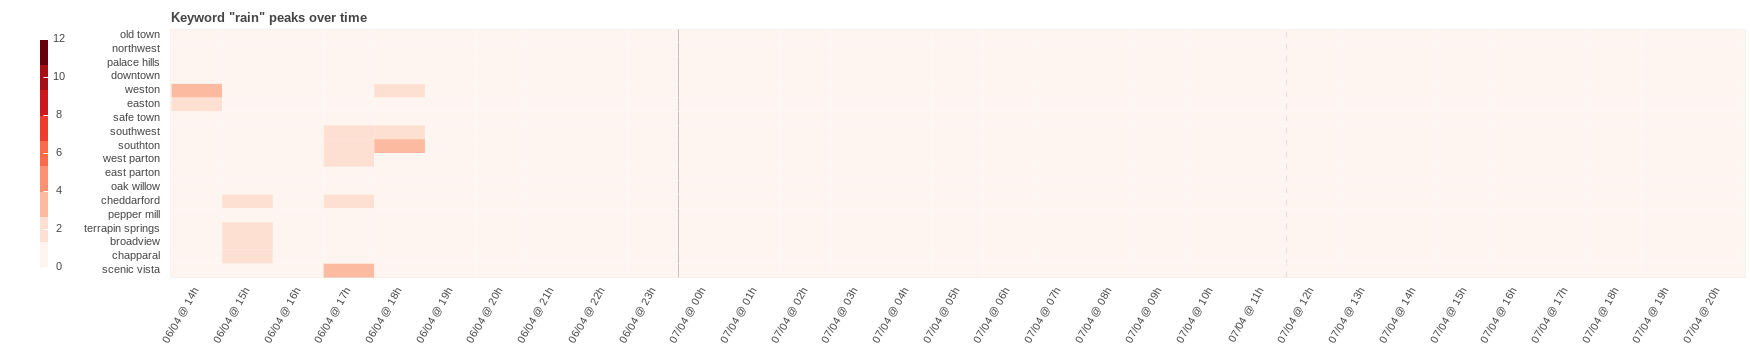
\includegraphics[width=1.00\textwidth]{figs/q1/cond_30h/cond_30h_rain.png}
        \caption{Rain}
        \label{fig:rain_30h}
    \end{subfigure}
    \begin{subfigure}[!h]{0.24\textwidth}
        \centering
        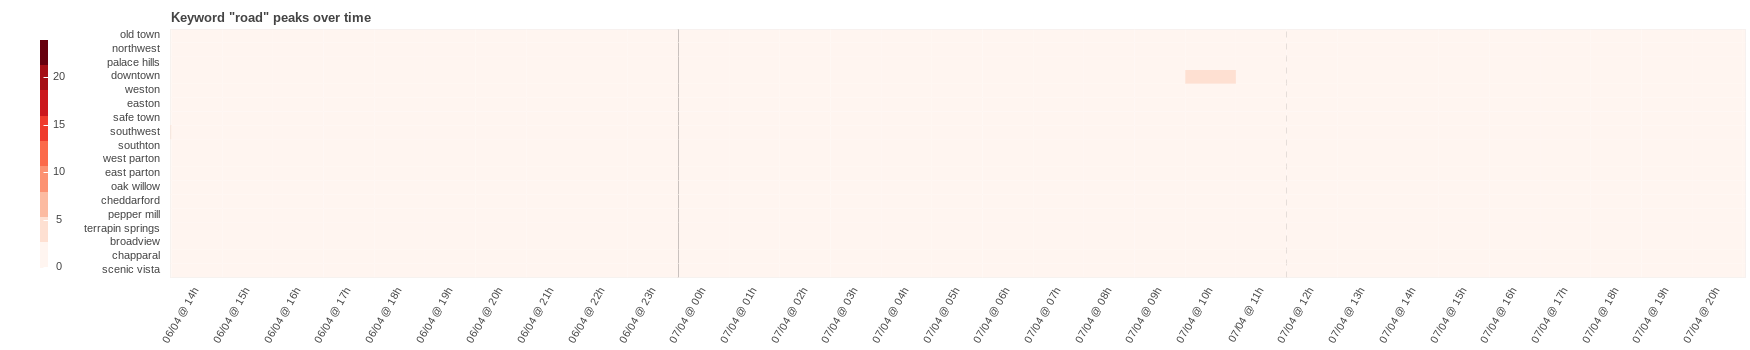
\includegraphics[width=1.00\textwidth]{figs/q1/cond_30h/cond_30h_road.png}
        \caption{Roads and Bridges}
        \label{fig:roads_30h}
    \end{subfigure}
    \begin{subfigure}[!h]{0.98\textwidth}
        \centering
        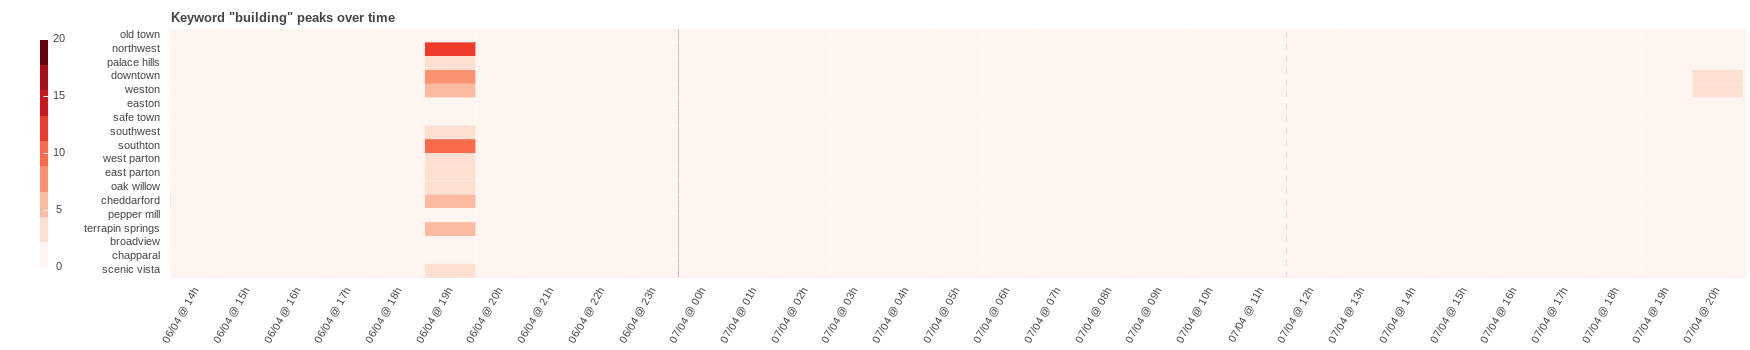
\includegraphics[width=1.00\textwidth]{figs/q1/cond_30h/cond_30h_build.png}
        \caption{Building}
        \label{fig:building_30h}
    \end{subfigure}
    \begin{subfigure}[!h]{0.98\textwidth}
        \centering
        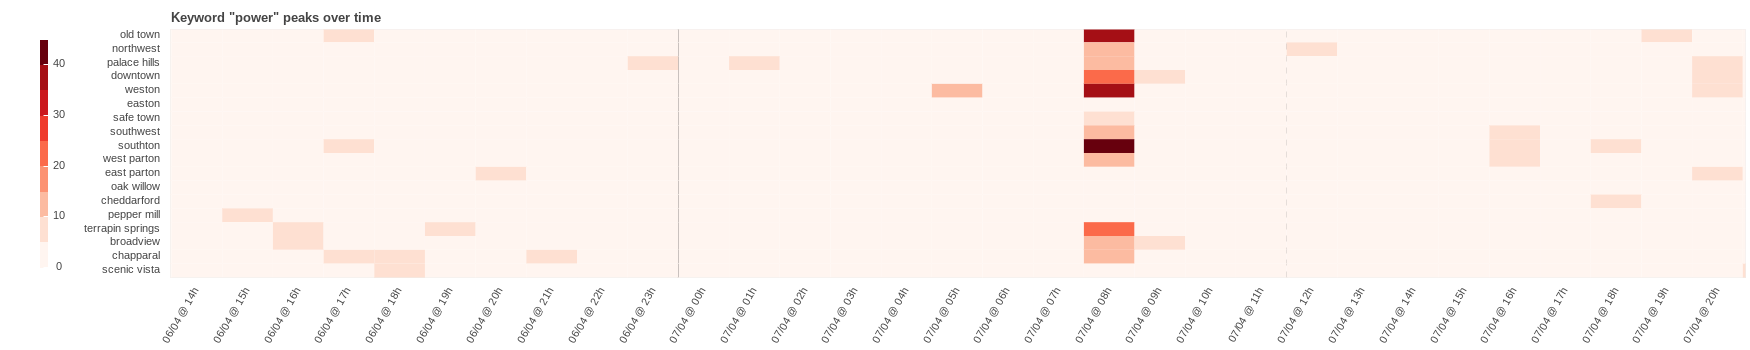
\includegraphics[width=1.00\textwidth]{figs/q1/cond_30h/cond_30h_power.png}
        \caption{Power}
        \label{fig:power_30h}
    \end{subfigure}
    \caption{Conditions after 30h of the first earthquake}
    \label{fig:eq_cond_30h}
\end{figure}

By looking at the heatmap of Figure~\ref{fig:eq_cond_30h} for each keyword, it
can be seen that there have been no occurrences for medical, and the ones
related to sewer/water and rain have already been attended within the first five
hours. With respect to roads and bridges in particular, there have been 3
occurrences from 10:00~AM to 11:00~AM of April 8th at Downtown, but this
neighbourhood is under resurfacing maintenance, which implies a road crew is
already working there.

Suggestions for crew allocation is detailed as follows:

\begin{itemize}
    \item \emph{Building}: On April 7th from 7:00~PM to 7:59~PM there have been
    multiple casualties on almost all locations so we would prioritize the
    dark-red-colored ones according to the heatmap of
    Figure~\ref{fig:building_30h}:
    Northwest, Southton, Downtown, and Weston. All four have a high 
    density of buildings and people, apart from being geographically close to
    each other, which can be an advantage for an eventual reallocation of crews
    in the following hours. Terrapin Springs and Cheddarford also have some
    less-intense occurrences, but they must be ignored due to the absence of
    high buildings.
    \item \emph{Power}: According to Figure~\ref{fig:power_30h} on April 7th 
    there have been sporadic, less-intense
    occurrences that could be solved by sending small units to individual
    locations, but from 8:00~AM to 9:00~AM an energy disaster appear to have
    affected almost all neighbourhoods. Again we would prioritize regions where
    the keywords were mentioned the most: Southton, Old Town, and Weston. The
    other can be later attended in the following hours.
\end{itemize}
%%% EOF %%%
